\documentclass{../../PublicResources/DocClass}

    \DocumentTitle{「计算机维修」学习笔记}
    \DocumentCreatedDate{2020/3/4}

    \LinkBlogPost{}
    \LinkPDFSource{}
    \LinkVideo{}

    \AuthorName{Mr. Kin}
    \AuthorEmail{im.misterkin@gmail.com}
    \AuthorBlog{https://mister-kin.github.io/}

\begin{document}
    \pagenumbering{Roman} % 大写罗马字母样式页码。
    \maketitle
    \addcontentsline{toc}{chapter}{封面}
    \frontmatter
    \phantomsection
\begin{center}
    {\bfseries\sffamily\Large 关于作者}
\end{center}
\addcontentsline{toc}{chapter}{关于作者}

\subsection*{\bfseries \sffamily 关于我}
\begin{wrapfigure}[3]{L}{60pt}
    \vspace*{-20pt}
    \centering
    
\includegraphics{kin-logo}
\end{wrapfigure}
\textbf{Mr. Kin},广东客家仁,程序猿,CG和游戏爱好者,一枚极客。翻译UP主,个人UP主。不定时在B站直播日常:码代码,码博客,翻译,做视频,做教程。 ($\vartheta$$\bullet$\_$\bullet$)$\vartheta$ \hyperlink{follow}{\emph{(点击关注我!)}}

\subsection*{\bfseries \sffamily 开源建设}

\noindent {\bfseries \sffamily 开源软件的中文化翻译}

\begin{itemize}
    \item \href{https://docs.krita.org/zh_CN/}{Krita手册}:2018.8.5 - \href{https://crowdin.com/profile}{2019.4.23}
    \item \href{https://docs.blender.org/manual/zh-hans/latest/}{Blender手册}:2019.7.20 - \href{https://www.blendercn.org/5812.html?tdsourcetag=s_pctim_aiomsg}{2019.9.4} - 至今(\href{https://developer.blender.org/p/Mr_Kin/}{翻译维护})
\end{itemize}

\subsection*{\bfseries \sffamily \hypertarget{contact}{联系方式}}
\vspace*{-1ex}
\noindent {\footnotesize \color{red} \em 注:联系时请注明身份,谢谢!}

\begin{itemize}
    \item QQ:\href{tencent://AddContact/?fromId=45&fromSubId=1&subcmd=all&uin=2312463626&website=www.oicqzone.com}{2312463626}\emph{\color{red}(点击号码加好友)}
    \item 邮箱:2312463626@qq.com ; im.misterkin@gmail.com
\end{itemize}

\subsection*{\bfseries \sffamily \hypertarget{follow}{关注渠道}}
\vspace*{-1ex}
\noindent {\footnotesize \color{red} \em 注:点击文字即可跳转关注!}
\vspace*{-2ex}

\begin{figure}[htbp]
    \centering
    
\includegraphics[scale=0.2]{WechatOfficialAccounts.png}
\end{figure}
\vspace*{-4ex}

\begin{figure}[htbp]
    \centering
    \begin{minipage}[t]{0.2\textwidth}
        \centering
        \caption*{\href{https://mister-kin.github.io}{博客 - Blog}}
        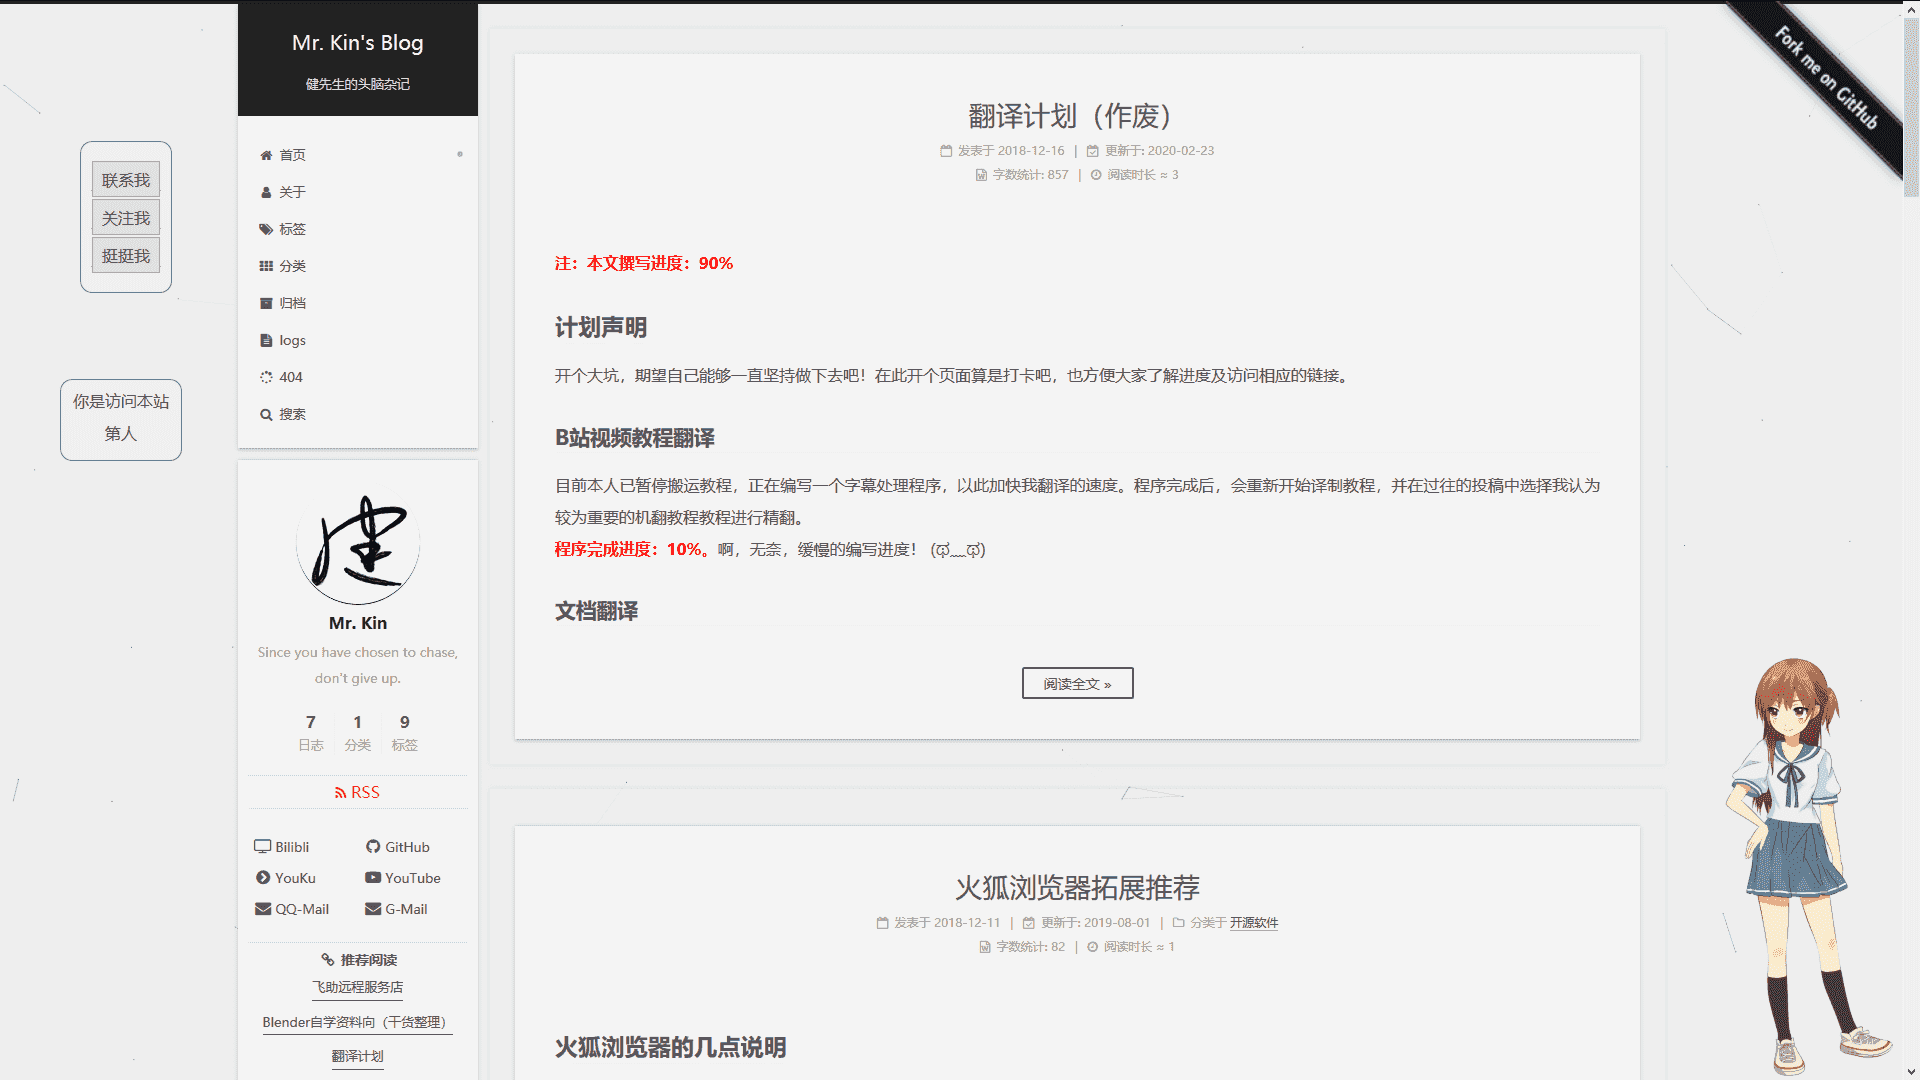
\includegraphics[scale=0.055]{Blog}
    \end{minipage}
    \qquad
    \begin{minipage}[t]{0.2\textwidth}
        \centering
        \caption*{\href{https://github.com/mister-kin}{Github}}
        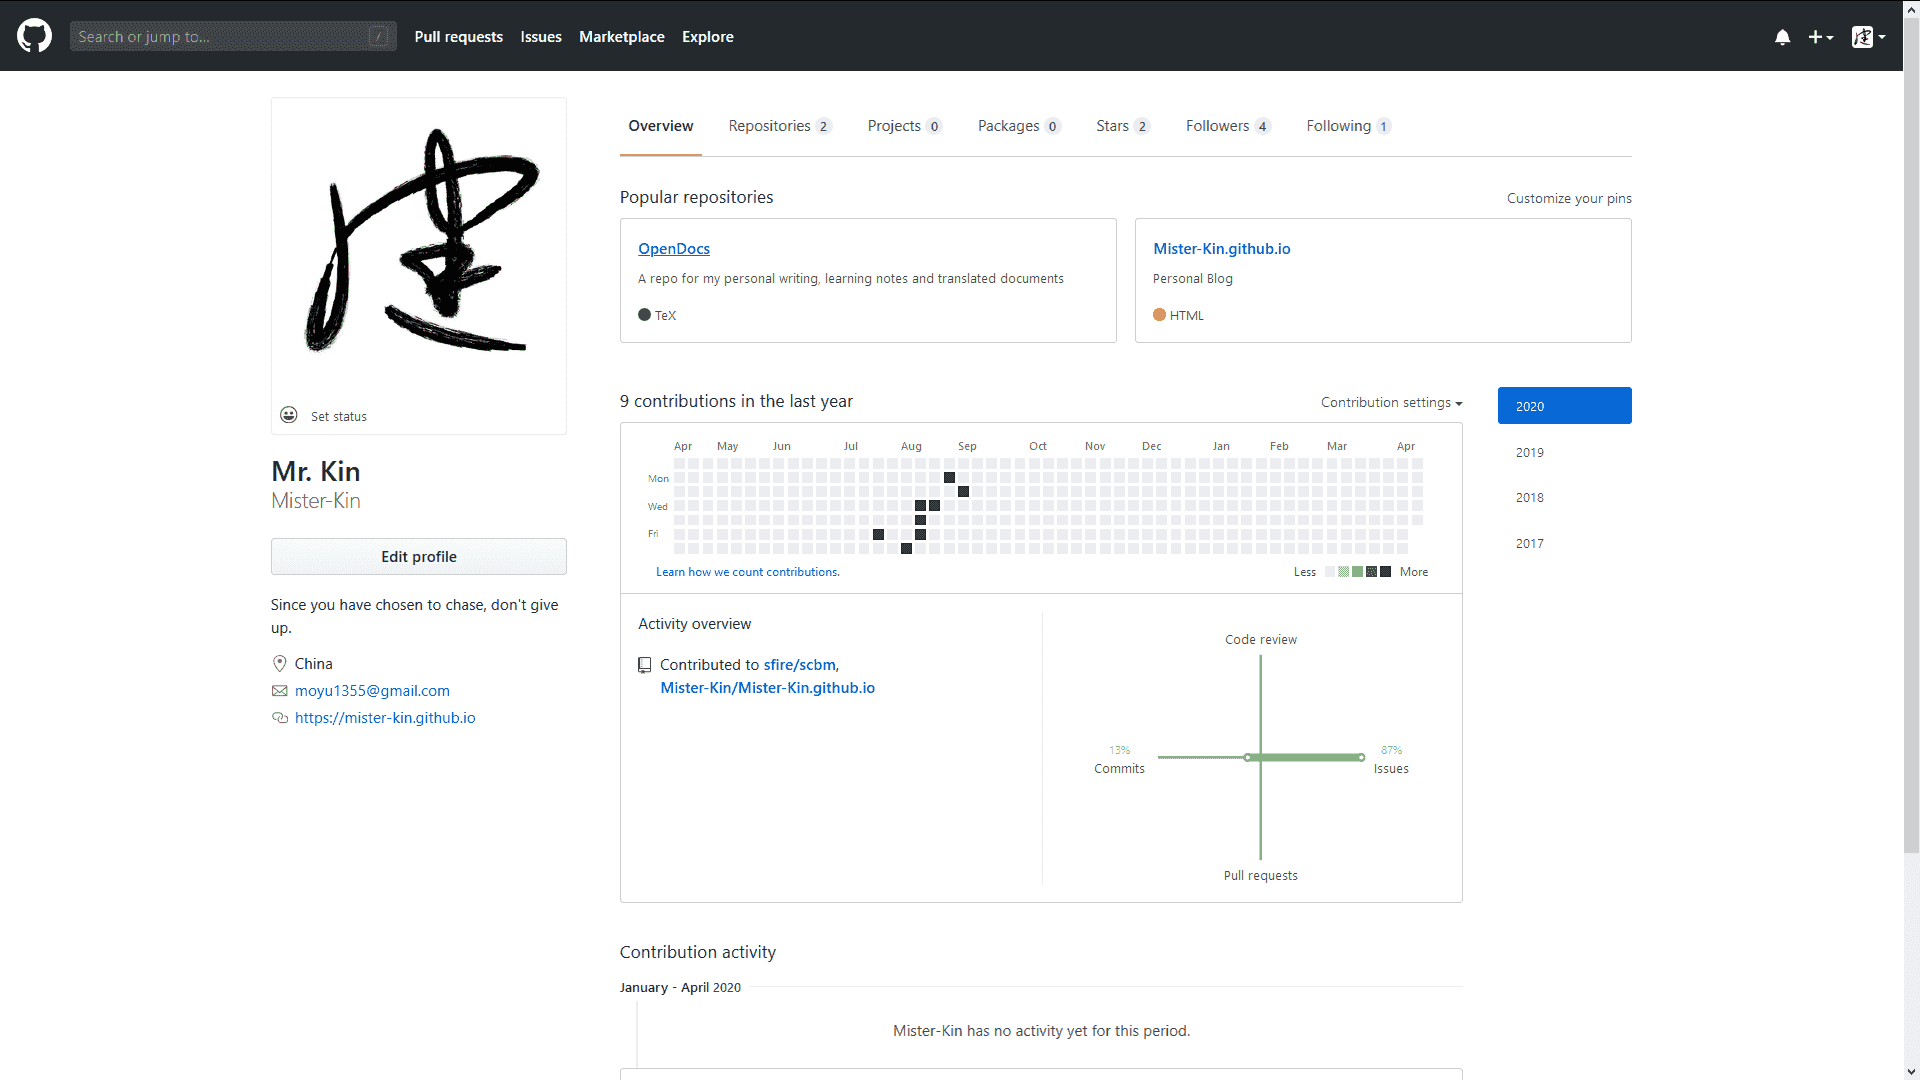
\includegraphics[scale=0.055]{Github}
    \end{minipage}
    \qquad
    \begin{minipage}[t]{0.2\textwidth}
        \centering
        \caption*{\href{https://weibo.com/6270111192/profile?topnav=1&wvr=6&is_all=1}{微博 - Weibo}}
        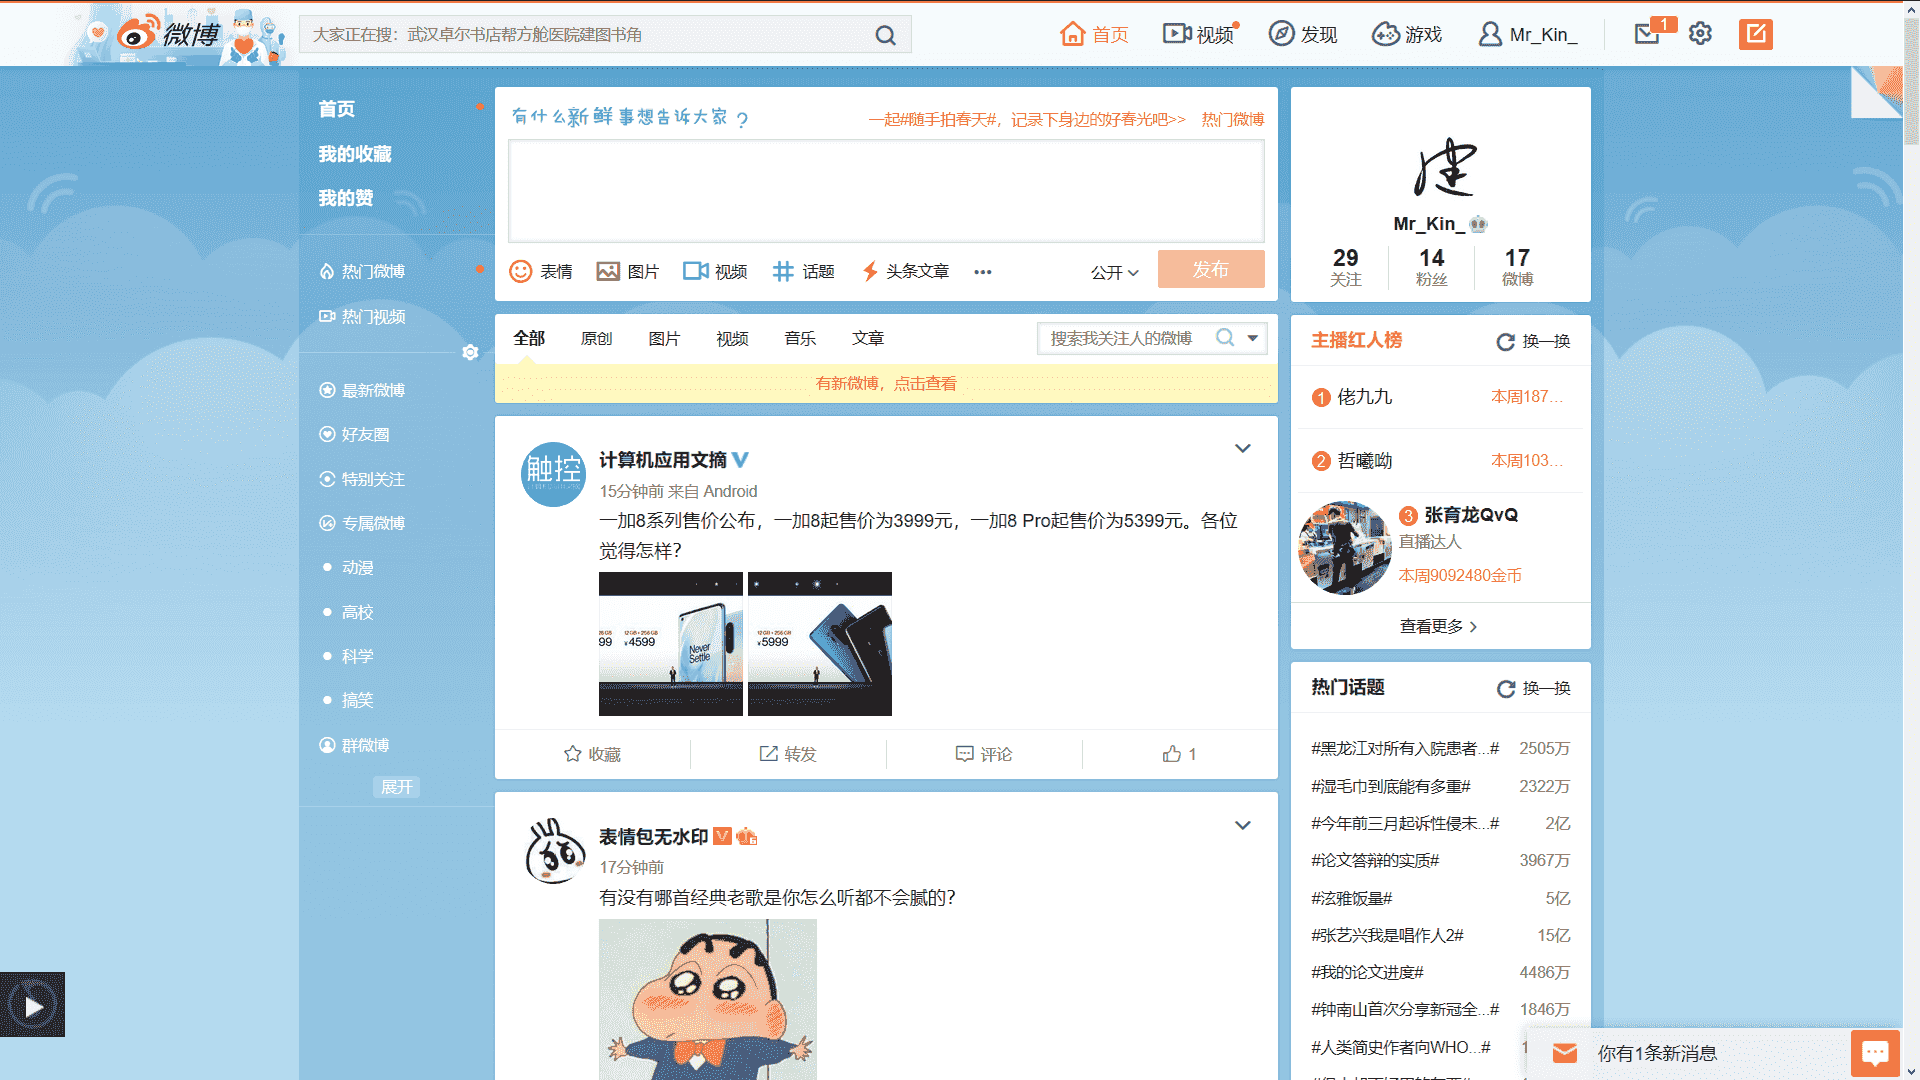
\includegraphics[scale=0.055]{Weibo}
    \end{minipage}
    \qquad
    \begin{minipage}[t]{0.2\textwidth}
        \centering
        \caption*{\href{https://www.zhihu.com/people/drwu-94}{知乎 - Zhihu}}
        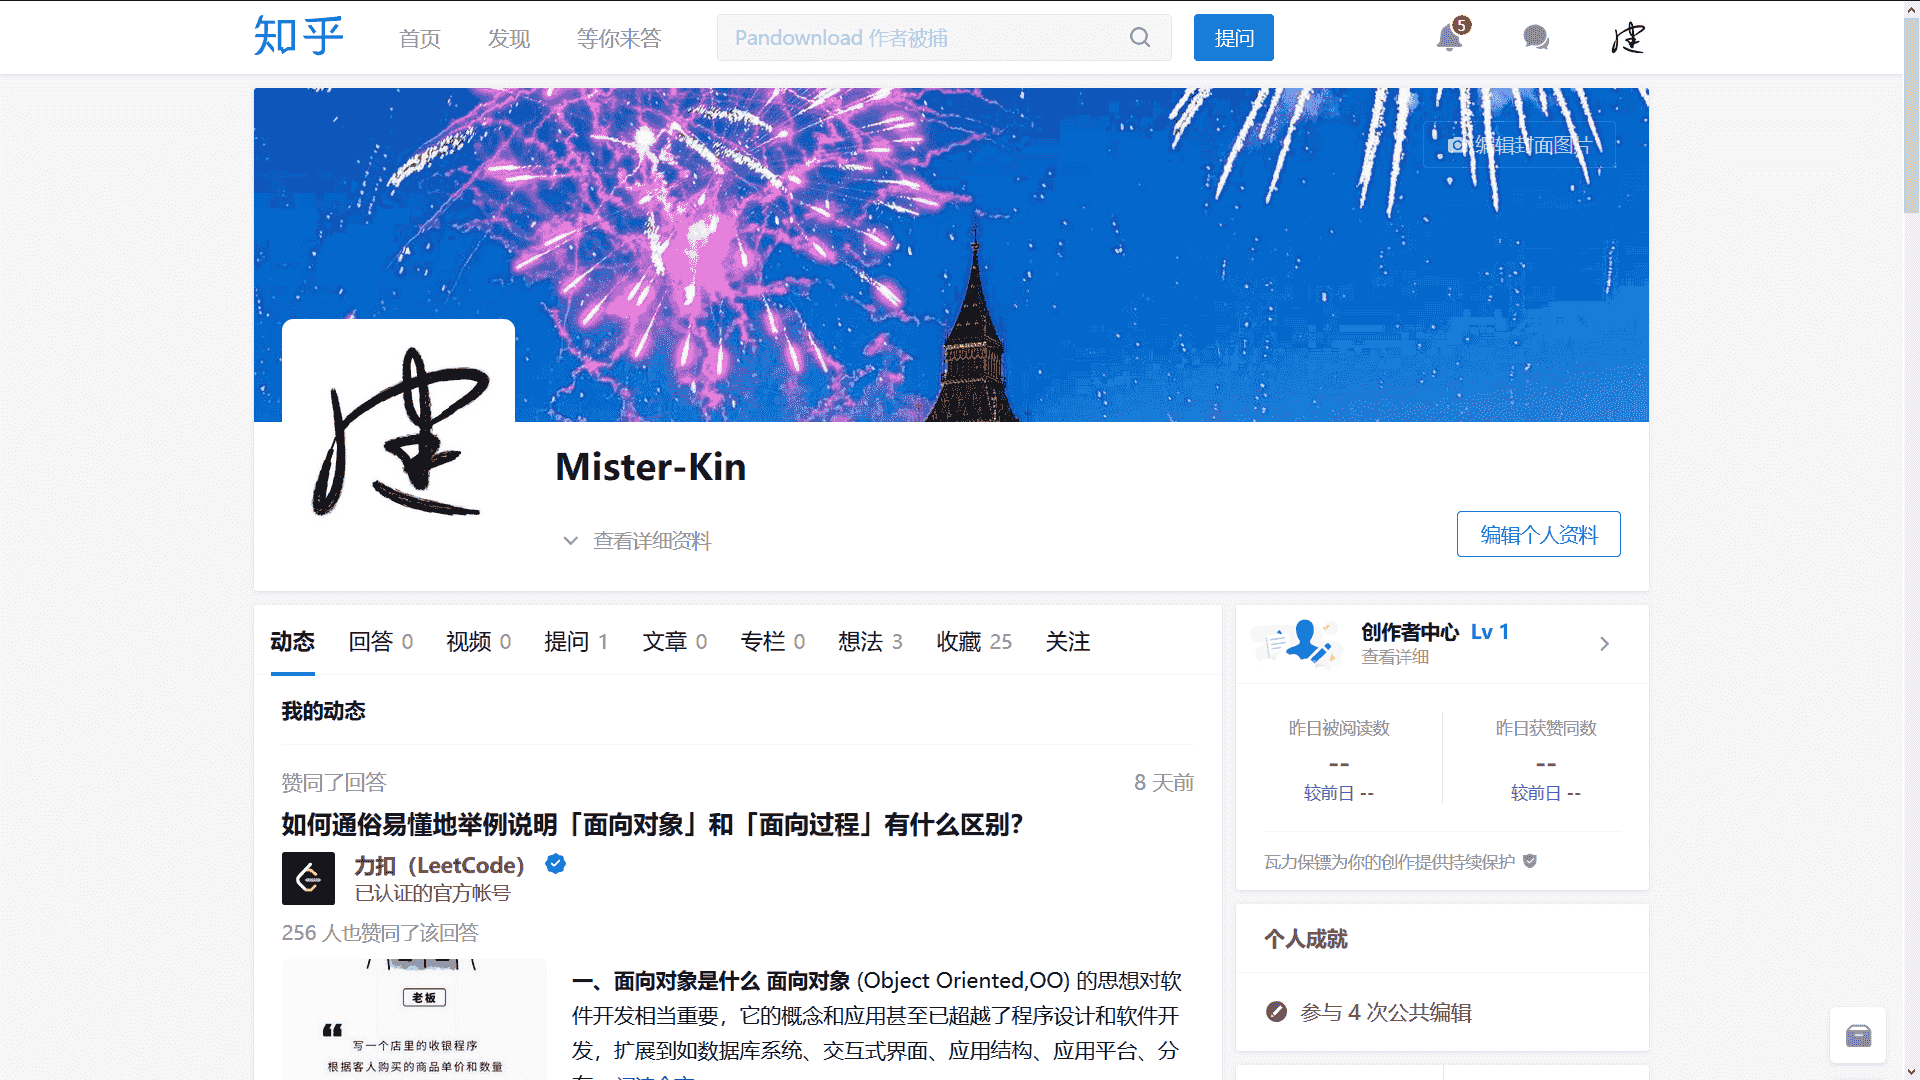
\includegraphics[scale=0.055]{Zhihu}
    \end{minipage}

    \vspace*{3ex}

    \begin{minipage}[t]{0.2\textwidth}
        \centering
        \caption*{\href{http://space.bilibili.com/17025250?}{B站 - Bilibili}}
        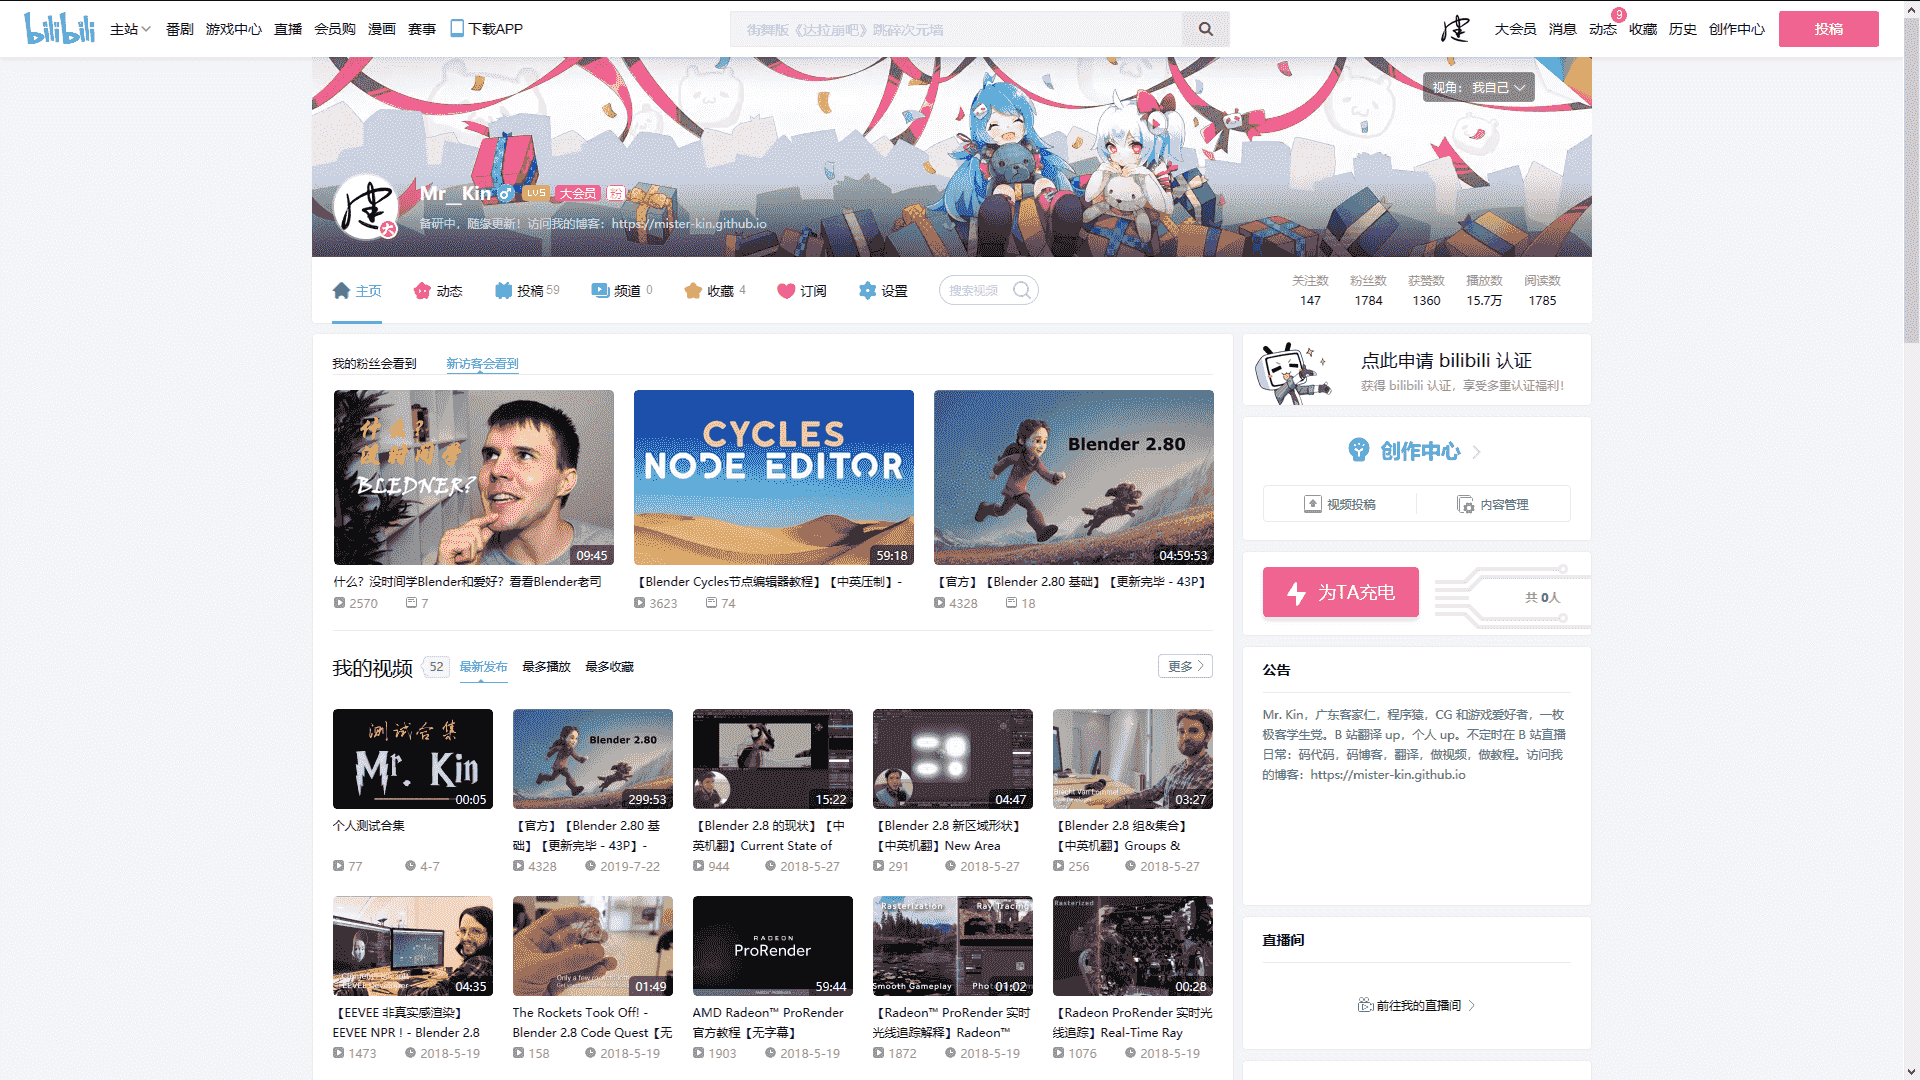
\includegraphics[scale=0.055]{Bilibili}
    \end{minipage}
    \qquad
    \begin{minipage}[t]{0.2\textwidth}
        \centering
        \caption*{\href{http://i.youku.com/i/UNjA3MTk5Mjgw?spm=a2hzp.8253869.0.0}{优酷 - Youku}}
        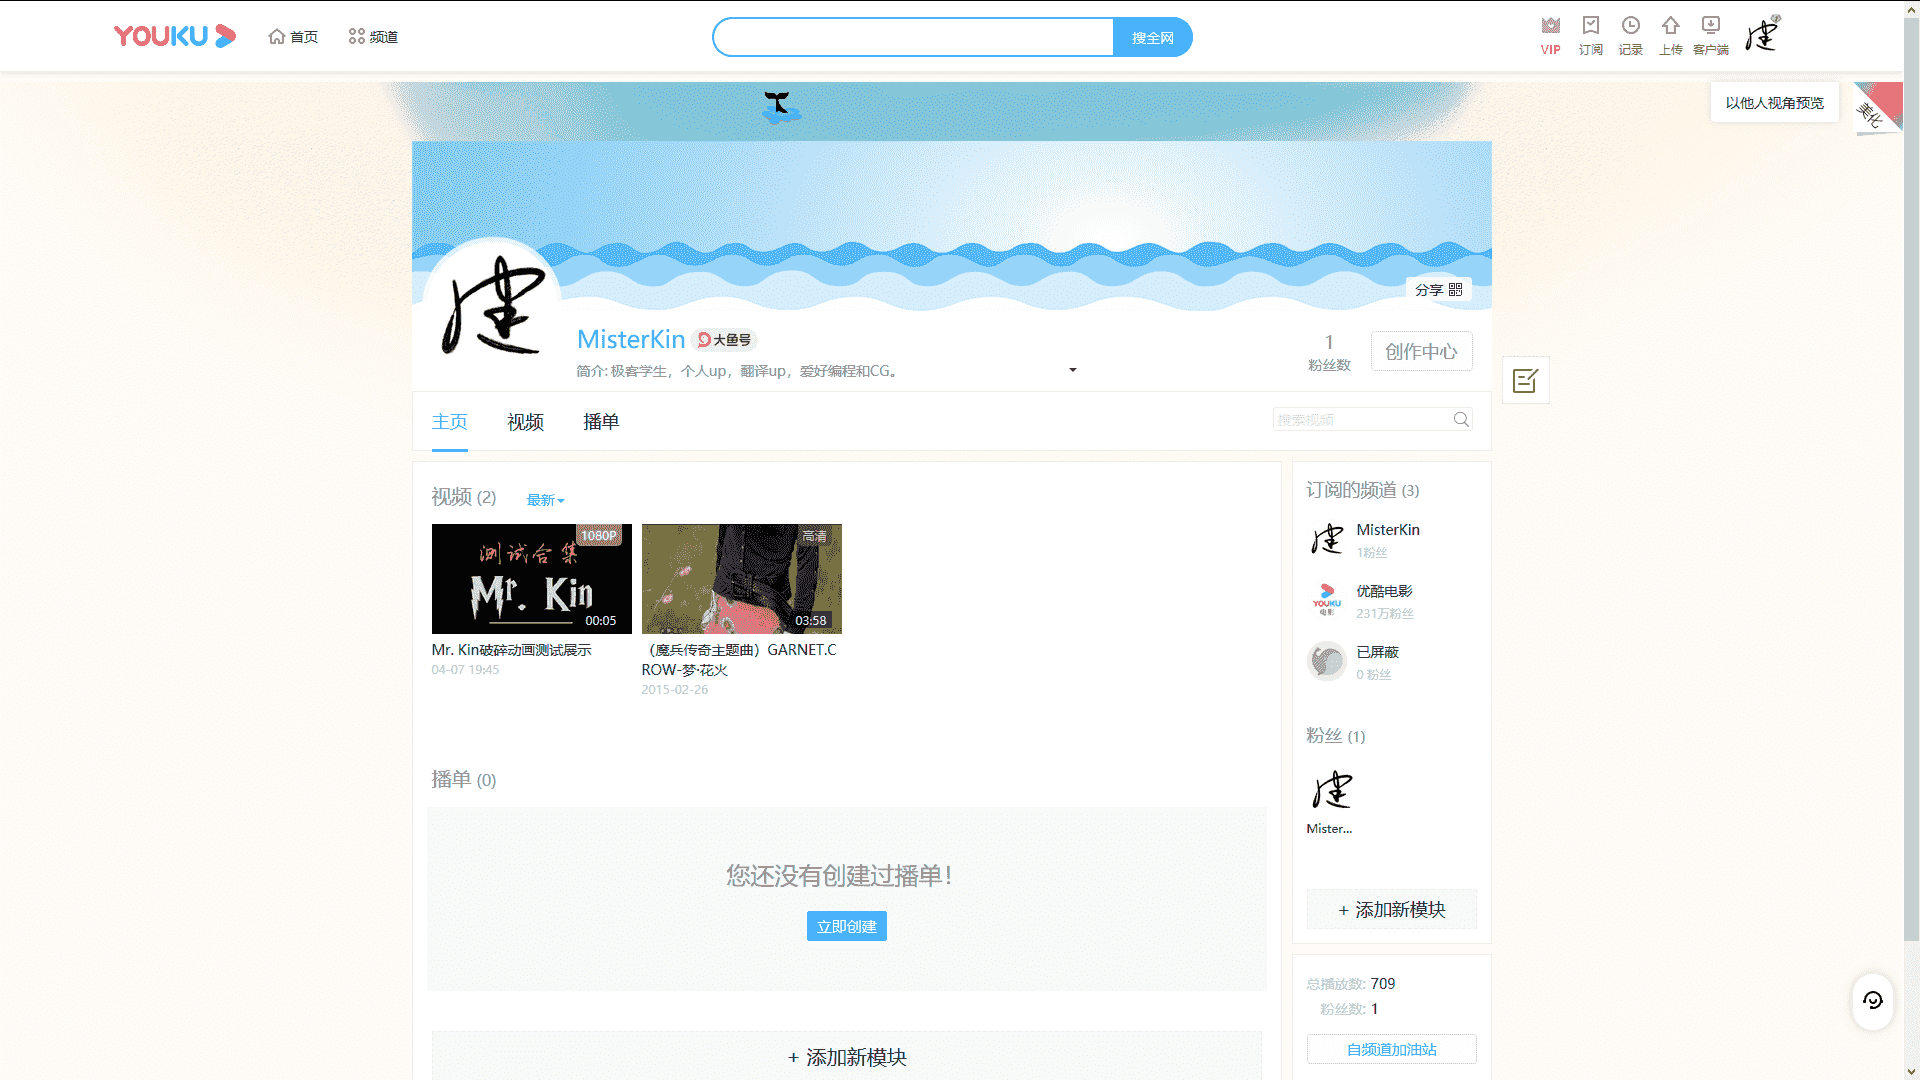
\includegraphics[scale=0.055]{Youku}
    \end{minipage}
    \qquad
    \begin{minipage}[t]{0.2\textwidth}
        \centering
        \caption*{\href{https://www.toutiao.com/c/user/835254071079053/\#mid=1663279303982091}{头条 - Headline}}
        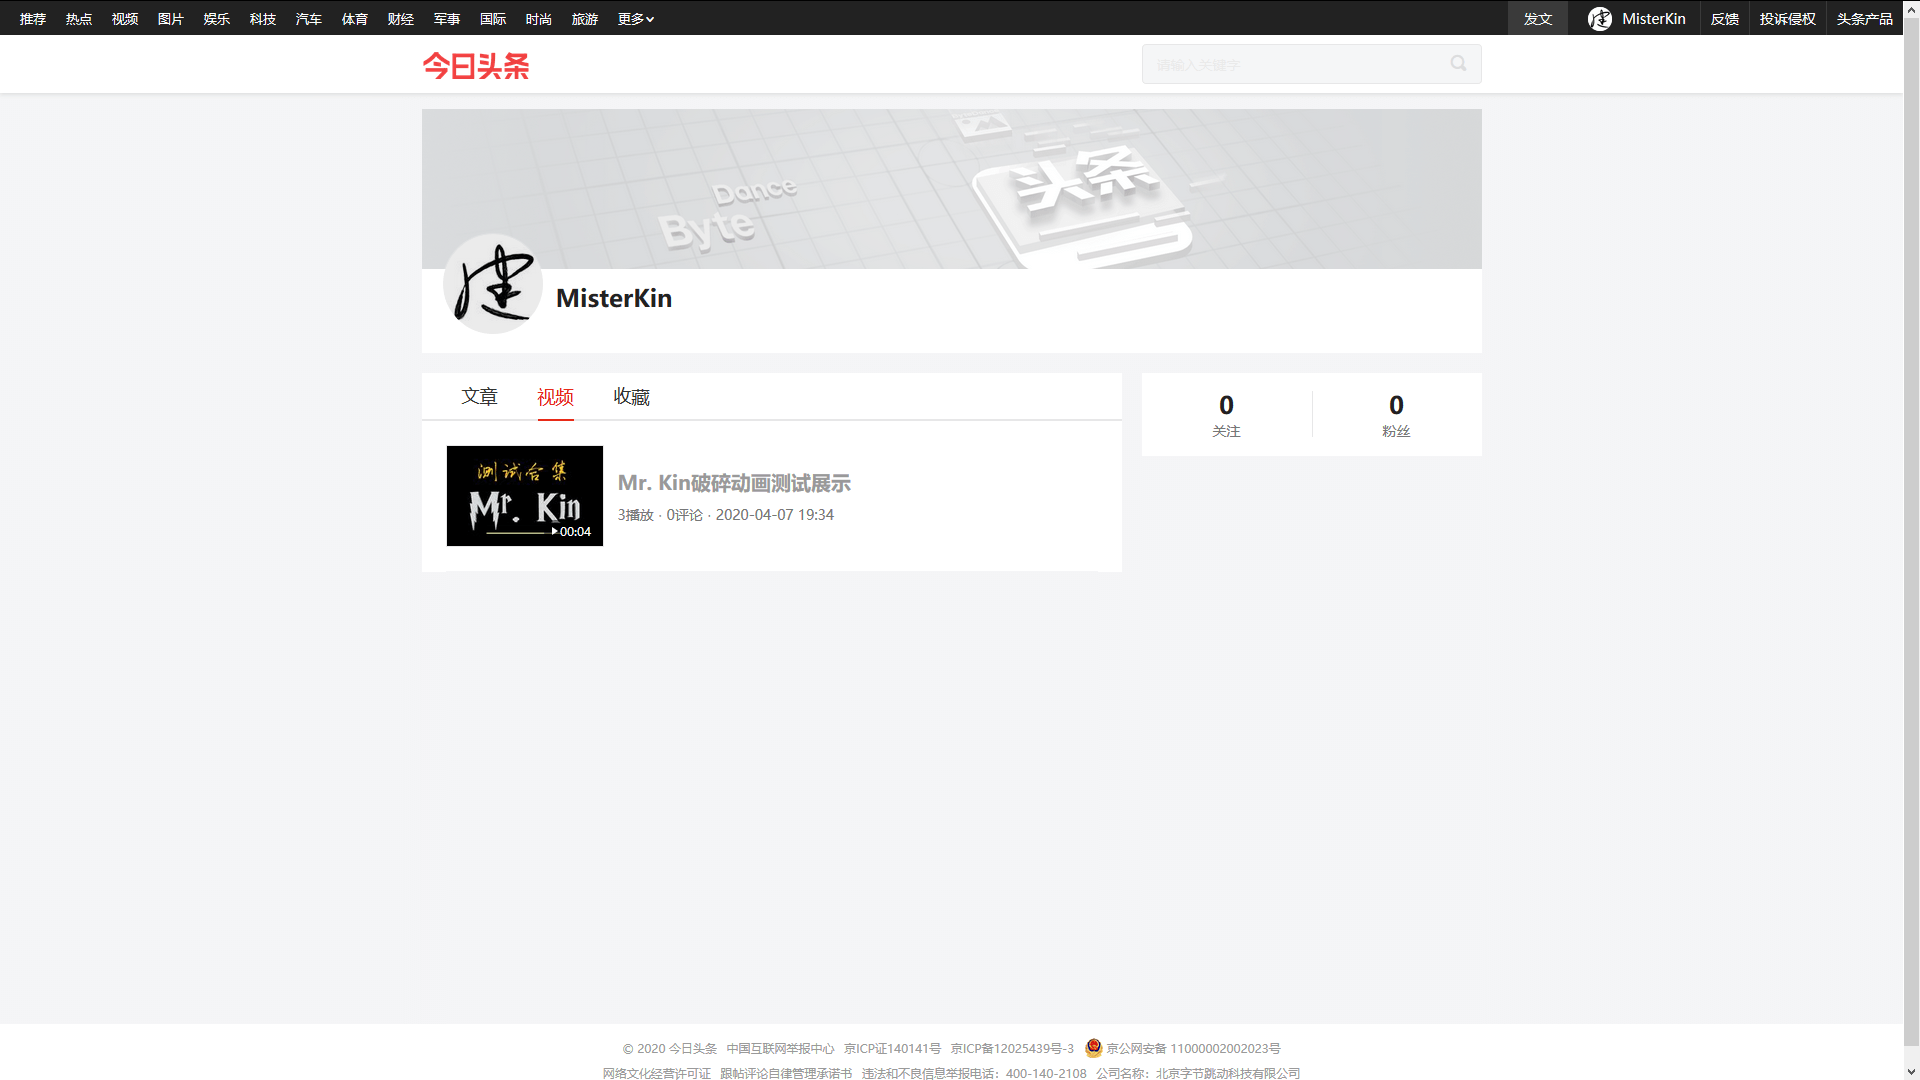
\includegraphics[scale=0.055]{Headline}
    \end{minipage}
    \qquad
    \begin{minipage}[t]{0.2\textwidth}
        \centering
        \caption*{\href{https://www.youtube.com/channel/UCXqjfWLzMlRKxGC8syWj17Q?view_as=public}{油管 - Youtube}}
        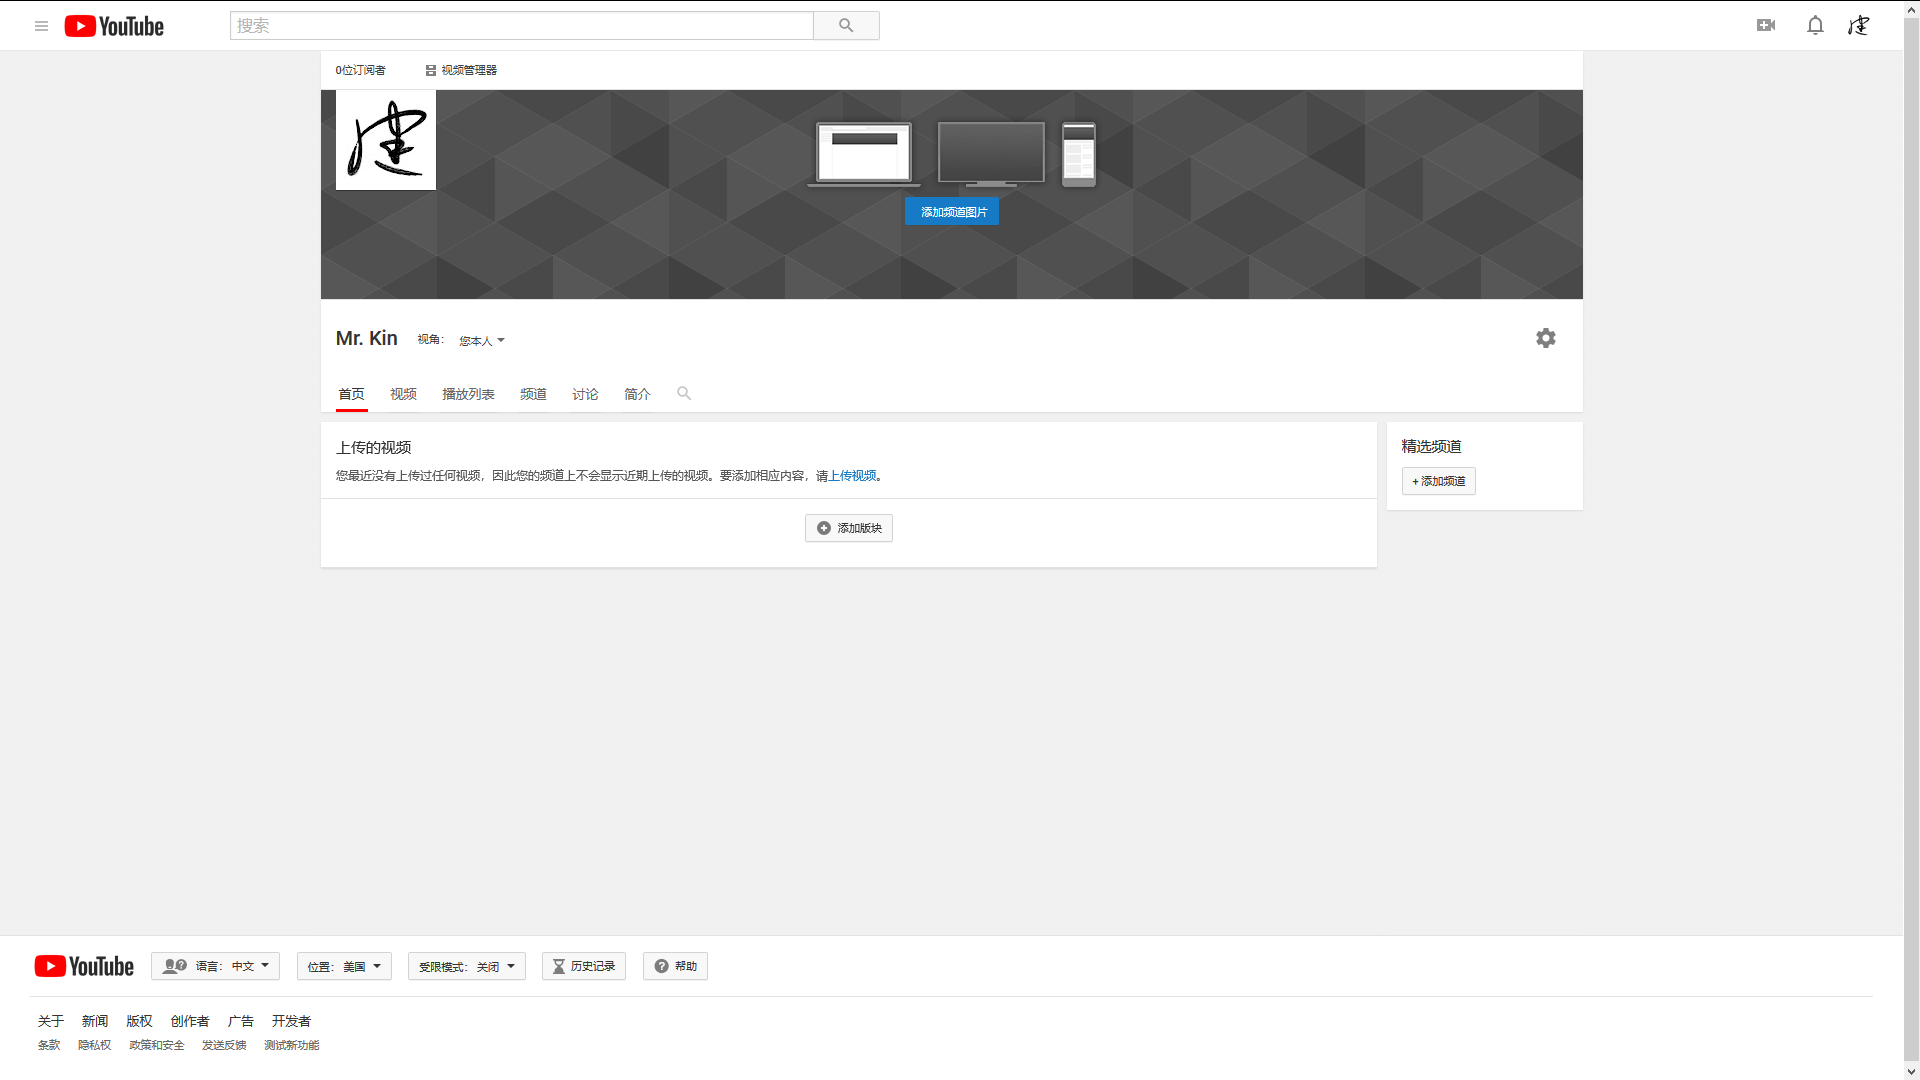
\includegraphics[scale=0.055]{Youtube}
    \end{minipage}
\end{figure}
 % 出于特殊的安全设置,\include 命令无法使用相对路径,因为需要读写权限以给 included file 写 aux 文件,而 \input 命令只需要读权限。
    \clearpage
    \phantomsection
\begin{center}
    {\bfseries\sffamily\Large 版权声明}
\end{center}
\addcontentsline{toc}{chapter}{版权声明}

\noindent 作者:Mr. Kin \\
\DetectToksEmpty\LinkBlogPost
\ifToksEmpty
博文链接:链接暂空\\
\else
博文链接:\href{\the\LinkBlogPost}{跳转博文页}\\
\fi
\DetectToksEmpty\LinkPDFSource
\ifToksEmpty
PDF及LaTex源码链接:链接暂空\\
\else
PDF及LaTex源码链接:\href{\the\LinkPDFSource}{跳转PDF及LaTex源码页}\\
\fi
\DetectToksEmpty\LinkVideo
\ifToksEmpty
\else
相关视频创作链接:\href{\the\LinkVideo}{跳转视频页}\\
\fi
许可协议:本作品的所有内容,除个人设计创作的图像(如logo等)和相关的视频创作及其他特别声明外,均采用\href{https://creativecommons.org/licenses/by-nc-sa/4.0/deed.zh}{知识共享\ 署名-非商业性使用-相同方式共享 4.0 国际许可协议}进行发布。版权 © Mr. Kin,保留所有权利。
\includegraphics[scale=.4]{CC-BY-NC-SA}\\*[1.3ex]
\begin{tabular}{|*{3}{p{0.306\textwidth}|}}
    \hline
    \textsf{\bfseries 允许} & \textsf{\bfseries 限制} & \textsf{\bfseries 条件} \\
    \hline
    \vspace{-8pt}{\color{green}√} 修改 & \vspace{-8pt}{\color{red}×} 商标使用 & \vspace{-8pt}{\color{blue}$\odot$} 保留原署名 \\[-12pt]
    {\color{green}√} 分发 & {\color{red}×} 专利使用 & {\color{blue}$\odot$} 状态变更说明 \\[-12pt]
    {\color{green}√} 个人使用 & {\color{red}×} 商业使用 & {\color{blue}$\odot$} 相同的许可和版权声明 \\
    \hline
\end{tabular}
\\*[1.3ex]
\emph{注:若想对本作品进行转载、引用亦或是进行二次创作时,请详细阅读上述相关协议内容(若不理解,请点击链接跳转阅读)。为保障本人权利,对于违反者,本人将依法予以处理!望周知!——Mr. Kin}

\begin{center}
    {\bfseries\sffamily\Large 勘误声明}
\end{center}

虽本人写作时已尽力保证其内容的正确性,但因个人知识面和经验的局限性以及计算机技术等相关技术日新月异,本作品内容或存在一些错误之处。还望诸君发现错误后能够\hyperlink{contact}{联系我}以更正错误,不胜感激!——Mr. Kin

\begin{center}
    {\bfseries\sffamily\Large 侵权声明}
\end{center}

若本作品采用的第三方内容侵犯了你的版权,请与我\hyperlink{contact}{联系}进行处理,谢谢!——Mr. Kin

\begin{center}
    {\bfseries\sffamily\Large 第三方开源许可声明}
\end{center}

\noindent 本作品使用的第三方开源产品有:
\begin{multicols}{2}
\begin{itemize}
    \item \href{https://github.com/adobe-fonts}{Adobe Fonts}: \href{https://github.com/adobe-fonts/source-serif-pro/blob/release/LICENSE.md}{OFL v1.1}
    \item \href{https://tug.org/texlive/}{Tex Live}: \href{https://tug.org/texlive/copying.html}{TeX Live Licensing}
    \item \href{https://code.visualstudio.com/}{Visual Studio Code}: \href{https://github.com/Microsoft/vscode/blob/master/LICENSE.txt}{MIT}
    \item \href{http://ffmpeg.org/}{FFmpeg}: \href{http://ffmpeg.org/legal.html}{LGPL v2.1 / GPL v2}
    \item \href{https://krita.org/en/}{Krita}: \href{https://docs.krita.org/en/KritaFAQ.html?highlight=license#license-rights-and-the-krita-foundation}{Krita's GPL license}
    \item \href{https://inkscape.org/}{Inkscape}: \href{https://inkscape.org/about/license/}{GPL}
    \item \href{https://www.gimp.org}{GIMP}: \href{https://www.gimp.org/about/COPYING}{GPL}
    \item \href{https://www.blender.org}{Blender}: \href{https://www.blender.org/about/license/}{GPL}
    \item \href{https://www.audacityteam.org/}{Audacity}: \href{https://www.audacityteam.org/about/license/}{GPL v2}
    \item \href{https://handbrake.fr}{Handbrake}: \href{https://github.com/HandBrake/HandBrake/blob/master/LICENSE}{GPL v2}
\end{itemize}
\end{multicols}

\noindent 更多请点击查看\href{https://mister-kin.github.io/about/third-party-declaration/}{第三方声明页}!

    \clearpage
    {\centering \tableofcontents} % 生成目录页。
    \mainmatter

    % 正文
    \chapter{笔记本基础}
\begin{intro}
    笔记本基础,板号,架构,名词解释。内容来源见
\end{intro}
\section{整体介绍}
\begin{tabular}{|*{5}{c|}}
    \hline
    外形 & A壳 & B壳 & C壳 & D壳 \\
    \hline
    位置 & 顶面的壳 & 屏幕面的外框 & 键盘面的壳 & 底面的壳 \\
    \hline
\end{tabular}

\section{部件介绍}
\subsection{PCB(印刷电路板)}

笔记本PCB集成度高,一般6层以上,比如6(较少),8,10\dots,不像1或2层板,无法跑线。板层数越多,EMI性能越好,成本也越高。

PCBA是指PCB上装配按照设定规则指定元件的成品功能板。(元件:电阻,电容,芯片,接口\dots)

注:PCB, Printed Circuit Board; PCBA, Printed Circuit Board Assembly; EMI, Electromagnetic Interference

\subsection{Chipset(芯片组)}
一般指南北桥。(目前北桥已逐渐淘汰)

常见厂商有:AMD,INTEL,NVDIA,VIA,SIS。

南桥:North Bridge Chipset,INTEL的为输出/输入控制器中心(Input/Output Controller Hub,ICH),NVIDIA的为MCP,ATI的称为IXP/SB,AMD的为FCH。
北桥:North Bridge Chipset,INTEL的为GMCH,Graphics \& Memory controller hub,带G有集显,无G的无集显。

\subsection{CPU(中央处理器)}
常见厂商:AMD,INTEL。龙芯,VIA,IBM,Transmeta。

不同芯片组对应不同的Intel CPU座(阵脚不同)

注:CPU, Center Processor Unit

\subsection{Battery(电池)}
组成:外壳+控制板+电芯。
类型:圆柱型、方型、聚合物
电芯:常见18650型锂离子电芯。单个电压3.7V,充电电压4.2V,电容量为2400mAH。三串两并:电压为3*3.7V,容量为2*2400mAH。

\subsection{Adapter(适配器)}
输入100~240V的AC(50/60Hz),输出16~20V居多。(华硕EPC有9.5V和12V的输出)

\section{笔记本和台式机的区别}
\begin{itemize}
    \item 笔记本自带显示系统(LCD/LED,专用屏线接口,自带高压板,灯管)
    \item 笔记本电源统一只由一个电压转出,常见16~20。台式主板由ATX电源提供12V、5V、3.3V等电压。\\这个是最大区别,笔记本的工作电压是由板子转换完成(16-20V主供电输入,经PWM电路降压处理,提供待机电压等工作电压),台式主板电源完成(多种方式,不只PWM)。
    \item 笔记本有充放电的电路,可用电池做替代电源。
    \item 为保证笔记本移动性和续航,CPU低功率、节能设计。
    \item 笔记本的保护电路多,过热保护,过电压保护。
    \item 笔记本内置鼠标设备,如指点杆,触摸板。
    \item 笔记本元件集成度高,MOS管多为8脚贴片。专用IC也多。(芯片功能作用原理类似,供电不是太复杂。)
    \item 笔记本6-8层板,夹层中也有信号线。台式主板4层,一般只在正反面有信号线。
    \item 笔记本引入EC(多功能芯片)概念,类似台式主板的IO,但功能更多,因为处理键盘的各种信号(亮度调节,声音调节等快捷键)。部分EC里会带有程序,其脚位功能由程序决定。
    \item 笔记本的时序概念很重要,电压和功能的实现,都由时序控制。环环相扣,前面条件未完成,后面动作就不会执行。
    \item 笔记本维修对电路图依赖很强,需要电路图分析陌生元件,且需要点位图对照。无这些的话,只能维修一些通病。(信号复杂,板子小,整合度高)
\end{itemize}

\section{笔记本板号}
板号:板子型号。即工程代号,Project Code

笔记本大规模的代工厂:广达(quanta),仁宝(compal),纬创(wistron),英业达(inventec),和硕联合(pegatron)。
二线代工厂:神达(mitac),蓝天(clevo),大众(fic),微星(msi),精英(ecs)

OEM代工:品牌商设计,代工厂生产。如苹果,联想(thinkpad)。成本高
ODM代工:设计和生产都是代工厂。

广达:DAO+板号+mb,一般为3个字,如ch3,zq5
仁宝:la-xxxxp
纬创:板号+mb(有白框)
华硕(asus): 板号+main board(没有位置号,PCB丝印层无标记,若无点位图无法分析)
英业达:板号(很长)+mb,一般给hp做得多
微星:ms-板号
富士康:代工索尼

\section{主板板子元件}
CPU座,北桥,南桥,内存插槽,独立显卡,显存,SPI BIOS,pice,电池接口,适配器插头,时钟芯片,ec,LCD接口,硬盘接口,键盘接口,光驱接口,读卡器槽。

\section{笔记本主板架构}
修接口。供电维修看架构没用。

intel双桥架构:
\begin{enumerate}
    \item CPU管理北桥。
    \item 北桥管内存,独显,显示接口,与cpu的连接的总线---FSB前端总线。北桥与南桥的总线---DMI+CLINK
    \item 南桥管理周边设备,网卡,迷你卡,USB,摄像头,EC,光驱,硬盘等,南桥和EC连接的总线--LPC总线,7根重要信号:LAD0,LAD1,LAD2,LAD3,LFRAME\#,LCLK,LRESET\#。(诊断卡接9根,外加VCC、GND)
    \item EC管理键盘,触控板,鼠标,部分挂BIOS(SPI ROM)
\end{enumerate}

intel单桥架构(无北桥):
\begin{enumerate}
    \item CPU管理显卡,内存。CPU不管显示接口,通过PCH桥到显示接口(cpu里有集成显卡,通过FDI总线输出)
    \item pch(管理原来南桥的功能)相比原南桥,增加了显示接口(VGA,LVDS,HDMI等)管理,可能也直接管理SPI rom(BIOS)
    \item EC管理键盘,温控芯片,触摸板,挂BIOS
\end{enumerate}

AMD(ATI)双桥架构:
\begin{enumerate}
    \item CPU管内存
    \item 北桥管理所有PCIE,显示接口。网卡(1000M,走PCIE)
    \item 南桥管理USB,网卡(100M,走PCI。),硬盘光驱等
\end{enumerate}

AMD单桥架构:
\begin{enumerate}
    \item CPU管理内存,显卡,显示接口(这个是与intel的区别)
    \item 桥(fch)管理网卡,mini-pcie,硬盘光驱,USB,EC,声卡等
    \item EC管键盘,鼠标
\end{enumerate}

intel和AMD单桥架构无时钟芯片,集成在桥。nvidia的双桥和amd相同。nvidia单桥:CPU管内存,桥管其他。

\section{名词解释}
\begin{intro}
    复位和PG都是测电压,时钟是测频率(无示波器时,可测电压,33MHz大概1.6V,100MHz大概0.4V)。
\end{intro}
\subsection{供电和信号}
\subsubsection{供电}
供电一个可以输出电流的电压,电流较大。工作过程中,这个电压不能置高或拉低。供电被拉低,就是短路。一般,也不许置高。(动力来源)。

常见有19,12,5(往上大电压给接口),3.3(给芯片),2.5,1.8,1.5,1.25,1.05,1.2,1.1,0.9,0.75V。CPU供电0.7-1.5V

名称一般为:VCC,VDD,VCC3,VDDQ,VTT,VBAT,5VALW,+3VO等(有V字)。苹果的供电特殊,例如PP0V75\_s3\_mem

符号为一个圆圈,T型,三角形。表示固定的电压,不允许置高和拉低。信号电压(例如19V)与1.5V(供电)碰在一起会变为1.5V。

\subsubsection{接地}
接地是给供电构成回路。有接地,才会有电流流过设备。

名称一般为:VSS、GND。

符号:三角形(数字地);倒三角形多横线(模拟地)。避免数字和模拟连在一起相互干扰。例子:数字地和模拟地通过一个0欧姆电阻PR170(值0\_6),实际测量是通路,但信号不一样。如果这个0欧姆电阻坏了,可能导致烧元件。压差相对值不一样。

\subsubsection{信号}
理论上,电压信号值考虑电压变化,电流很小。在工作过程中,可根据需要置高或者拉低。电路图中的信号的箭头不完全代表信号的流向,因为画图人员的随意性。
信号方向考经验判断:例如PWRBTN\#给南桥的;slp\_s3\#南桥出来的;therm\_stp\#温控信号看情况:过温时,温控芯片吧温控信号拉低。

\subsection{高低电平}
数字逻辑电路中,高电平表示1,低电平表示0。一般规定:低电平为0-0.25V,高电平为3.5-5V。

主板中,1V以上为高电平,0.7以下为低电平。

结论:根据电路判断高低电平,非限定特定值。有些电路0.5就是高,有的电路1.1还是低。但0肯定是地,3.3肯定是高。

\subsection{脉冲和跳变}
上升沿,下降沿。

类型:高电平跳变为低电平;低电平跳变为高电平;高跳变为低再跳变为高。

\subsection{时钟信号}
时钟信号CLK(Clock的简写)。为数字电路工作提供一个基准,使各个相连设备统一步调工作。单位Hz。南桥晶振323.768KHz。

主板上都有一个主时钟产生电路,给所有设备提供时钟,送出到cpu的频率为100MHz以上,送给PCI的是33MHz,送给PCIE的是100MHz,送给USB控制器(集成在南桥内部)的为48MHz。

相连的两个设备需要相同的时钟频率和电压才能通信,如内存和北桥。

时钟信号需要在主板正常通电后且时钟芯片工作正常才能测量到,用示波器和万用表(测电压?)测。100M的示波器一般测不了CPU的频率。

\subsection{复位信号}
复位信号RST(RESET的简写)。复位都是从高电平向低电平跳变再回到高电平,如PCI的复位是从3.3V向0V跳变再回到3.3V就是一个正常的复位跳变。

名称一般为:xxxRST\#,如PCIRST\#、CPURST\#、IDERST\#等。复位只能是瞬间低电平,主板正常工作时复位都是高电平。但不是恒高电平,不能直接接到供电上。如台式机reset键,复位开关弹不起来就一直为低电平,就不行。

平常说没复位,通常指没复位电压,即复位信号测量点电压为0V。维修一般都是把复位电压修出来。

所有设备的复位信号,如EC,北桥等,都是由南桥发出。开机的瞬间,便会对设备清零,使其重新工作。

\subsection{PG信号}
电源好信号PG(powergood的缩写),用来描述供电正常的信号。一般高电平有效。如cpu供电芯片,只有在正常发出cpu电压后,才会发出PG信号。

名称一般为:PG、PWRGD、PWROK、POK、PWRG、VTTPWRGD、CPUPWRGD等。

\subsection{开启信号}
开启信号。有的芯片叫EN(enable),使能,高电平时表示开启信号。有的芯片叫SHDN\#(shutdown),\#表示低电平有效。综合名称和\#来看,意思是低电平时关闭芯片,高电平开启。所以一般shutdown信号一般要维持高电平。

注:信号带\#时(低电平有效),一定要结合信号的英文全程去理解。有的带\#,为低电平时主板可以正常工作。例如:VT\_PWRGD\_CK410\#信号是cpu供电正常后发出低电平开启时钟信号。1999\_SHDN\#信号是低电平关闭MAX1999的控制信号,即为高电平时,主板才能正常工作。

    \chapter{维修工具}
\section{可调电源}
检测电流,电压。接入机器才会显示电流。可剪断电源正极的通用口线,自己做一个开关。(防止弄坏电源机械开关,有些机器待机电流也偏大,不宜频繁开关?)

通用口可接特定的接口,可接不同厂商的机器。

\section{烙铁}

\section{热风枪}

\section{万用表,打值卡,假负载,诊断卡}

\section{示波器}
主要是供电和信号,不是频率

\section{BGA返修台}


    \nocite{*} % 不使用 cite 也能生成参考文献。
    \printbibliography % 生成参考文献排版。
    \addcontentsline{toc}{chapter}{参考文献} % 添加参考文献进目录。

    \appendix
    % 附录

\end{document}
